%-------------------------------------------------------------------------------
% Autores: I. R. Pagnossin e Centro de Ensino e Pesquisa Aplicada.
%
% Este material é parte integrante do curso "Usando LaTeX; pensando em TeX" e é
% distribuido pelos autores segundo a licença Creative Commons 2.5 Brasil
% (atribuição/não-comercial/redistribuição segundo a mesma licença).
%
% This material is part of the course "Usando LaTeX; pensando em TeX".
% It is distributed according to the license Creative Commons 2.5 Brazil
% (atribution/non-comercial use/share alike the same license).
%-------------------------------------------------------------------------------
\newif\ifhandout
%\handouttrue  % Descomente se for para gerar a versão para IMPRESSÃO.
\handoutfalse % Descomente se for para gerar a versão para APRESENTAÇÃO

%-------------------------------------------------------------------------------
\ifhandout
 \documentclass[handout]{beamer}
 \mode<handout>
\else
	\documentclass{beamer}
	\mode<presentation>
\fi

	\usepackage[utf8]{inputenc}
	\usepackage{fourier}	
	\usepackage[brazil]{babel}	
	\usepackage{graphicx}
	\usepackage{listings}
	\usepackage{tikz}
	\usepackage{helvet}	
	\usepackage{amsmath}
	
	\ifhandout
		\usepackage{pgfpages}
		\pgfpagesuselayout{2 on 1}[a4paper,border shrink=5mm]
	\fi
	

	% Configurações pessoais
	% Configurações personalizadas do código LaTeX.	
\lstnewenvironment{LaTeXcode}{
	\setlength{\abovecaptionskip}{0pt}	
	\lstset{language=[LaTeX]TeX}
	\lstset{%
		basicstyle=\footnotesize\ttfamily,  % Global
		keywordstyle=\color{blue}\bfseries, % Comandos
		identifierstyle=,                   % Texto
		stringstyle=,                       % Strings 
		commentstyle=\color{gray},          % Comentários
		showstringspaces=false,             % Espaços
		rulecolor=\color{gray},             % Linha da caixa
	}
	\lstset{emph={setlength,includegraphics,psfrag,subfigure},emphstyle={\color{blue}\bfseries}}
}% Abrindo o ambiente.
{}% Fechando o ambiente.
	
\newcommand{\digite}[1]{{\fontfamily{cmss}\fontseries{bx}\selectfont#1}}	
\newcommand{\cs}[1]{{\normalfont\textbackslash\color{blue!50!black}#1}}
\newcommand{\pkg}[1]{{\normalfont\sffamily\color{orange}#1}}
\newcommand{\env}[1]{{\normalfont\sffamily\color{green!50!black}#1}}
\let\comando=\cs
\let\package=\pkg
\let\ambiente=\env
\newcommand{\foreign}[1]{{\textsl{#1}}}


	\newcounter{exercicio}	
	\newenvironment{exercicio}{%
		\refstepcounter{exercicio}%
		\penalty-200
		\noindent\colorbox{blue!60!black}{\makebox[\columnwidth-\fboxsep*2][c]{\textbf{\color{white}Exercício~\theexercicio}}}\smallskip
	}{\par\medskip}
		

\newcommand{\bibtex}{\textsc{Bib}\TeX}

\newenvironment<>{atividade}[1]{%
\begin{actionenv}#2%
\begin{exampleblock}{{Atividade #1}}%
}
{%
\end{exampleblock}%
\end{actionenv}%
}


	% Path das figuras, relativo a esta pasta.
	\graphicspath{{../arquivos_comuns/figuras/}{./figuras/}}

	% Modelo da apresentação	
	\usetheme{Frankfurt}
	\usefonttheme{serif,structurebold}
	
	% Metadados do arquivo PDF.
	\hypersetup{
		pdftitle={Origem do TeX/LaTeX e seus prós e contras},
		pdfauthor={Dr. Ivan R. Pagnossin},
		pdfsubject={LaTeX},
		pdfkeywords={TeX,LaTeX}
	}

	% Título, autores e instituição.
	\title{Introdução}
	\author{\textbf{Prof.:} Ivan R. Pagnossin \and \textbf{Tutora:} Juliana Giordano}
	\institute{%
		Coordenadoria de Tecnologia da Informação\\
		Centro de Ensino e Pesquisa Aplicada}
	\logo{
\includegraphics[width=0.25\textwidth]{LogotipoCursoLaTeX_v3_pequeno}}
	\date{}
	
	
\begin{document}

	\newsavebox{\knuthpicture}
	\savebox{\knuthpicture}{\raisebox{-\height}[0pt][0pt]{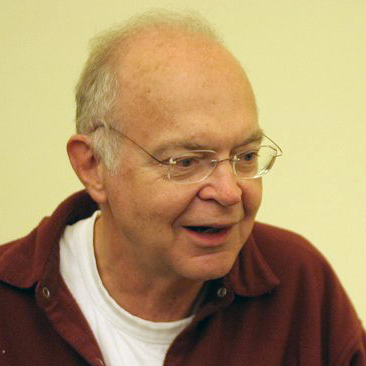
\includegraphics[width=0.2\textwidth]{DonaldEKnuth}}}
	\newsavebox{\lamportpicture}
	\savebox{\lamportpicture}{\raisebox{-\height}[0pt][0pt]{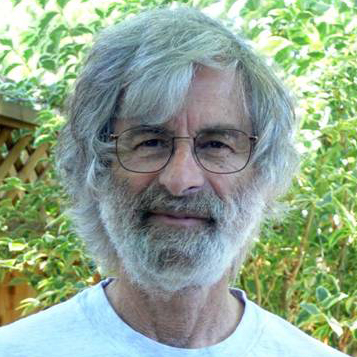
\includegraphics[width=0.2\textwidth]{LeslieLamport}}}

%-------------------------------------------------------------------
\begin{frame}[label=titulo]
	\centering
		
	
\includegraphics[width=0.8\textwidth]{LogotipoCursoLaTeX_v2}

	\titlepage
\end{frame}

%-------------------------------------------------------------------
\section{O que é o \LaTeX?}
\begin{frame}
	\frametitle{O que é o \LaTeX?}

	\begin{quote}
	``\LaTeX\ é um sistema para a composição de documentos (\dots)\\	
	tornou-se a `língua-padrão' no mundo científico.''\par
	\end{quote}\par\vspace{\baselineskip}
	\hfill Laslie Lamport\qquad\null\\
	\hfill {\scriptsize em \textsl{\LaTeX: a document preparation system}}\qquad\null{\scriptsize\par}
	
\end{frame}

\setbeamertemplate{background canvas}
		{
\includegraphics[width=\paperwidth,height=\paperheight,keepaspectratio=false]{leao-pensador-wattermark.png}}

%-------------------------------------------------------------------
\logo{} % <-- O logotipo não aparecerá mais a partir daqui.

\section[Origem]{A origem do \TeX\ e do \LaTeX}

\begin{frame}[shrink=1]
	\frametitle{Origem}
		
	\begin{block}{\TeX}<1->
		\begin{minipage}[t]{0.7\textwidth}
			\begin{itemize}
				\item<1-> Tipografia digital
				\item<2-> Donald E.~Knuth, entre 1977 e 1983
				\item<3-> Do grego {$\tau\epsilon\chi\nu\eta$}: ``arte'' e ``tecnologia''
				\item<4-> Pronuncia-se ``téc'' (?)
				\item<5-> Escreve-se \textsf{TeX}
			\end{itemize}
		\end{minipage}\hfill
		\begin{minipage}{0.2\textwidth}
			\onslide<2->{\usebox{\knuthpicture}}
		\end{minipage}
	\end{block}
	
	\begin{block}{\LaTeX}<6->
		\begin{minipage}[t]{0.7\textwidth}
			\begin{itemize}
				\item<6-> Pacote de macros do \TeX
				\item<7-> Leslie \alert<7>{La}mport, em 1985
				\item<8-> Pronuncia-se ``latéc'' ou ``leitéc'' \quad \hyperlink{engracado}{
\includegraphics[width=2ex]{smiley}}
				\item<9-> Escreve-se \textsf{LaTeX}
				\item<10-> \emph{O pulo do gato}: organização lógica
			\end{itemize}
		\end{minipage}\hfill
		\begin{minipage}{0.2\textwidth}
			\onslide<7->{\usebox{\lamportpicture}}
		\end{minipage}		
	\end{block}	
\end{frame}
%-------------------------------------------------------------------

\section{Prós e contras}
\subsection{Vantagens}

\begin{frame}
  \frametitle{Vantagens do \LaTeX}

  \begin{itemize}
  \item<+-> Integração entre texto e expressões matemáticas \quad \hyperlink{word}{
\includegraphics[width=2ex]{smiley}}
  \item<+-> Incorpora princípios tipográficos (ff, fi etc)

  \item<+-> Comunidade (documentação, progresso e ajuda)

  \item<+-> É estável e requer pouco hardware
  \item<+-> Distribuições \TeX/\LaTeX\ para Windows, Unix, Mac OS etc
  \item<+-> Arquivos \TeX/\LaTeX\ são portáveis e duradouros  
  
  \item<+-> Agilidade na edição: mouse $\times$ teclado
  \item<+-> \alert<8>{Organização lógica}
  \item<+-> Referências cruzadas
  \item<+-> Referências bibliográficas  
  \item<+-> Índice remissivo  
  \item<+-> Preço: \alert<12>{zero!}
  \end{itemize}  
\end{frame}

%-------------------------------------------------------------------
\subsection{Desvantagens}
\begin{frame}
	\frametitle{Desvantagens}

	\begin{itemize}
	\item<+-> Curva de aprendizagem
	\item<+-> Legibilidade do arquivo \textsf{tex}\dots
	\item<+-> \dots\ particularmente das tabelas
	\item<+-> Necessita de outras ferramentas (Ghostview, Ghostscript etc)
	\item<+-> Pré-visualização
	\item<+-> Diversidade de distribuições:
		\begin{itemize}
			\item<+-> \textsf{teTeX} para Unix (obsoleto)
			\item<+-> \textsf{TeX Live} e \alert<11>{\textsf{MikTeX}} para Unix e \alert<11>{Windows}
			\item<+-> \textsf{OzTeX} e \textsf{MacTeX} para Mac Os\\ etc
		\end{itemize}
	\item<+-> \alert<10>{Organização lógica}
	\end{itemize}
	
	\begin{center}
		\begin{uncoverenv}<11>
			\scriptsize
			Uma grande vantagem do MikTeX sobre o TeX Live é que seus pacotes podem\\
			ser obtidos	diretamente da Internet, à medida que forem requisitados.\par
		\end{uncoverenv}
	\end{center}
	
\end{frame}

%---------------------------------------------------------
\section{Organização lógica}
\subsection{Definição}

\begin{frame}
	\frametitle{Organização lógica}
	\framesubtitle{Definição}	
	
	\centering\Huge
	\pause
	\textbf{Organização lógica} é aquela baseada na \emph{função} dos elementos de um contexto.
		
\end{frame}

%---------------------------------------------------------
\begin{frame}%\transdissolve[duration=0.2]
	\frametitle{Organização lógica}
	\framesubtitle{Definição}
	
	\centering
	
	\begin{block}<1->{No MS Word e cia\dots \hfill WYSIWYG}
		\begin{minipage}[c]{0.25\textwidth}
			\centering
			\begin{tikzpicture}
				\fill[red,fill opacity=0.5] (0,0) circle (1);
				\fill[yellow,fill opacity=0.5] (0.5,0) circle (1);
				\node [label=above:Conteúdo] at (-1,0.8) {};
				\node [label=above:Leiaute] at (+1.5,0.8) {};
			\end{tikzpicture}
		\end{minipage}\hfill
		\begin{minipage}[c]{0.5\textwidth}\scriptsize
				\dots o autor desenvolve o conteúdo e define o leiaute simultaneamente. Por conseguinte,
				eles são fortemente correlacionados, de modo que alterações num deles afeta
				consideravelmente o outro.
		\end{minipage}
	\end{block}
	
	\begin{block}<2->{No \LaTeX\dots \hfill WYSIWYM}
	\begin{minipage}[c]{0.25\textwidth}
		\begin{tikzpicture}
			\fill[red,fill opacity=0.5] (0,0) circle (1);
			\fill[yellow,fill opacity=0.5] (1.5,0) circle (1);
			\node [label=above:Conteúdo] at (-0.5,0.8) {};
			\node [label=above:Leiaute] at (+2,0.8) {};
		\end{tikzpicture}
	\end{minipage}\hfill
	\begin{minipage}[c]{0.5\textwidth}\scriptsize
		\dots o autor desenvolve o conteúdo, deixando o leiaute por conta do \LaTeX. Neste paradigma,
		a correlação entre o conteúdo e o leiaute é fraca, embora não nula, de modo que alterações 
		num deles geralmente \emph{não} afeta o outro.\\[\baselineskip]
		{\tiny\textbf{obs.:} o \TeX\ \emph{não} é logicamente organizado.}
	\end{minipage}
	\end{block}	
\end{frame}

%-------------------------------------------------------------------
\subsection{Exemplo}
\begin{frame}
	\frametitle{Organização lógica}
	\framesubtitle{Exemplo 1}
	
	\begin{minipage}[t]{0.45\textwidth}
		\centering
		\onslide<1->{\Large\cs{emph}}\\[\baselineskip]
		\onslide<2->{\emph{Texto enfatizado}}\\
		\onslide<5->{\textbf{Texto enfatizado}}\\
		\onslide<6->{\textsc{Texto enfatizado}}\\
		\onslide<7->{\underline{Texto enfatizado}}
	\end{minipage}\hfill
	\begin{minipage}[t]{0.5\textwidth}
		\centering
		\onslide<3->{\Large\cs{textit}}\\[\baselineskip]
		\onslide<4->{\textit{Texto em itálico}}
	\end{minipage}
	
	\vfill
	
	\begin{uncoverenv}<8->\centering
		\small Entenda: um trecho de texto pode ser enfatizado de várias formas. O que\\
		não muda é o fato	de que este trecho \emph{é destacado} daquele ao seu redor.\par
	\end{uncoverenv}
\end{frame}

%-------------------------------------------------------------------
\begin{frame}[fragile]
	\frametitle{Organização lógica}
	\framesubtitle{Exemplo 2}
	
	\noindent{\bfseries\Large 5\quad Isto é uma seção?}
	\vspace{.5cm}\par	
	
	O texto acima pode até parecer uma seção, mas não é. Trata-se apenas de uma linha formatada à mão assim:
	\begin{uncoverenv}<2->
		\begin{LaTeXcode}	
		\vspace{.5cm}
		\noindent{\bfseries\Large 5\quad Isto é uma seção?}
		\vspace{.5cm}\par
		\end{LaTeXcode}	
	\end{uncoverenv}
	
	\onslide<3->{Uma seção de verdade\dots}
	\begin{itemize}
		\item<3-> é declarada assim pelo autor: {\bfseries\cs{section}\{Isto é uma seção?\}};
		\item<4-> é formatada pelo \LaTeX, não pelo autor;
		\item<5-> é acrescentada automaticamente no bookmarks;
		\item<6-> tem sua numeração automaticamente gerenciada;
		\item<7-> pode ser utilizada em referências-cruzadas.
	\end{itemize}	
\end{frame}

%-------------------------------------------------------------------
\section{Compilação}
\begin{frame}
	\frametitle{Compilação}
	\framesubtitle{Formatos \textsf{tex}, \textsf{dvi}, \textsf{ps} e \textsf{pdf}}
	
	\centering
		
	\mode<beamer>{%
		\includegraphics<2->[height=0.75\textheight]{compilacao_layer1}%
		\llap{\includegraphics<3->[height=0.75\textheight]{compilacao_layer2}}%
		\llap{\includegraphics<4->[height=0.75\textheight]{compilacao_layer3}}%
		\llap{\includegraphics<5->[height=0.75\textheight]{compilacao_layer4}}%
		\llap{\includegraphics<6->[height=0.75\textheight]{compilacao_layer5}}%
	}
	\mode<handout>{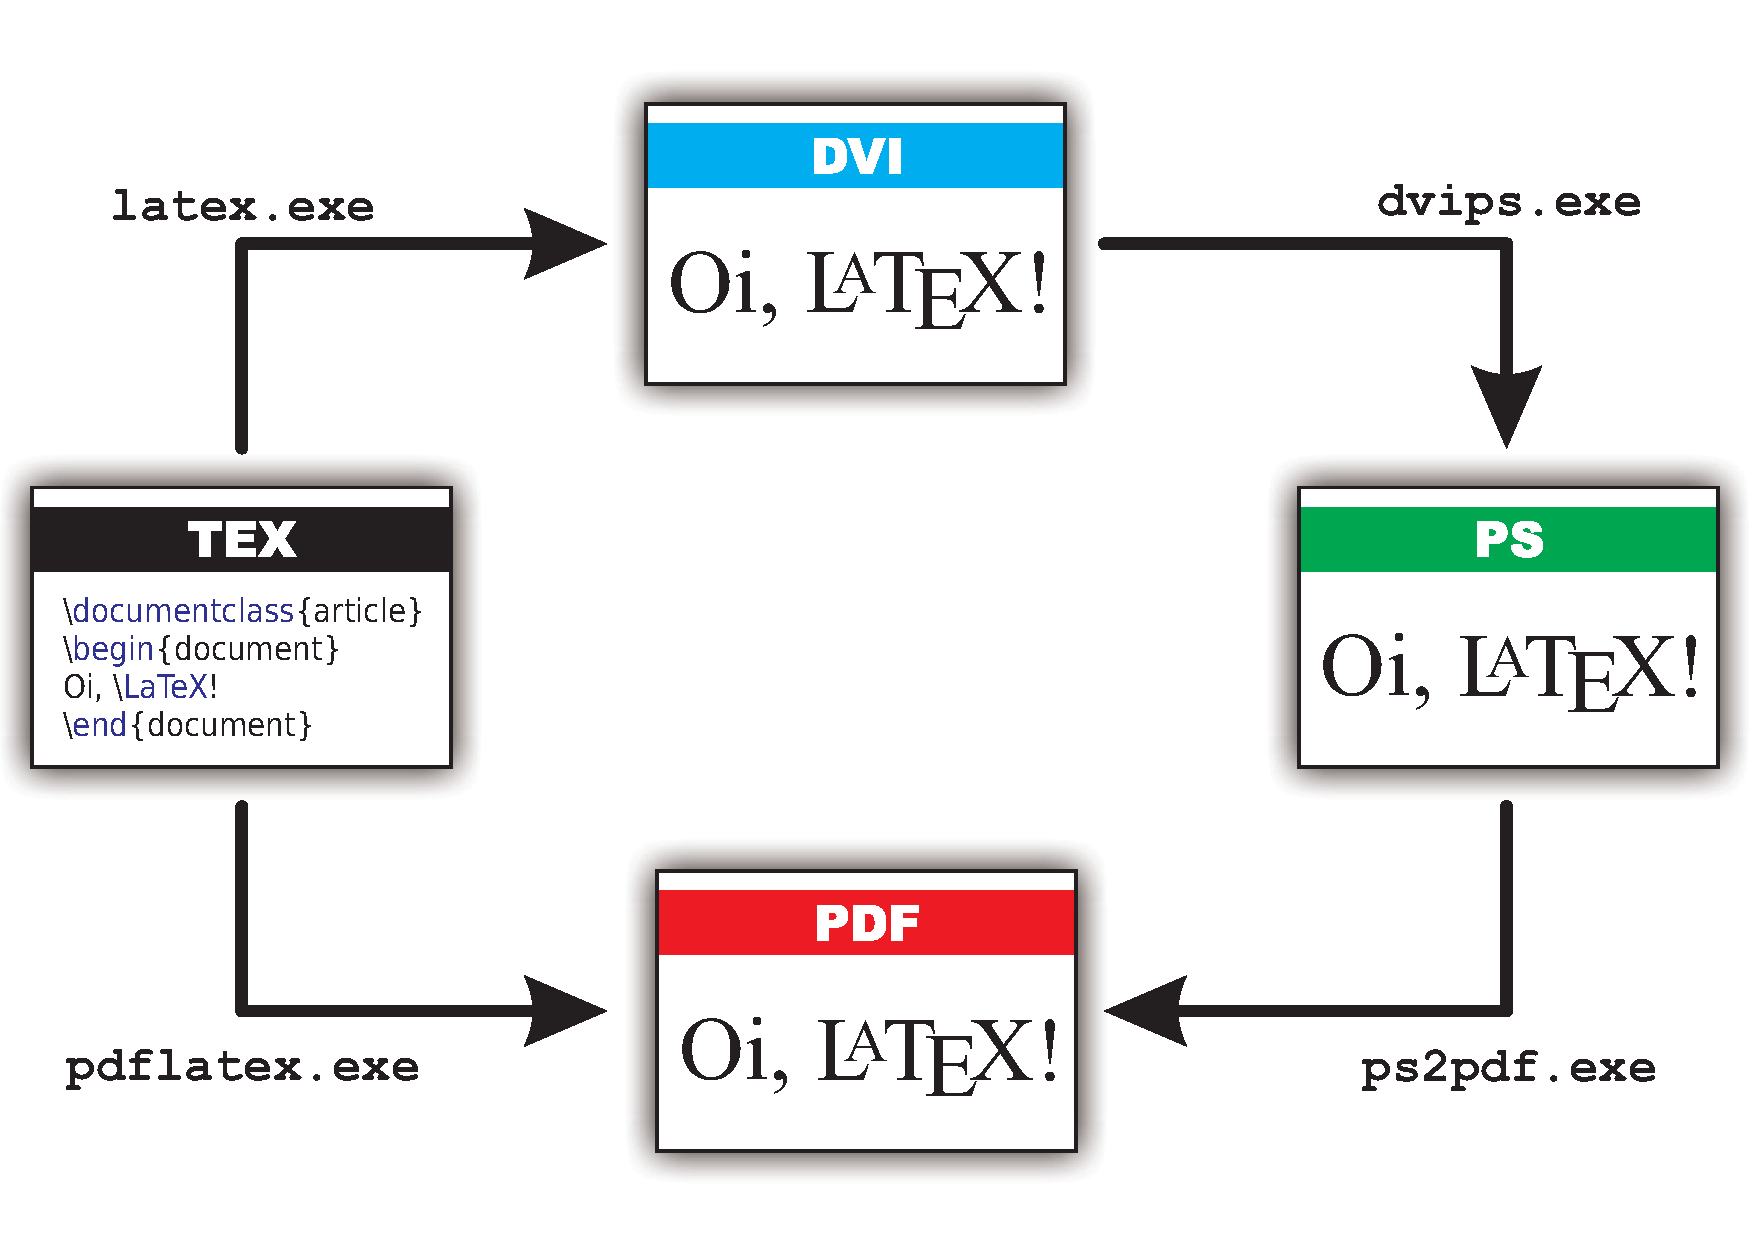
\includegraphics[height=0.75\textheight]{compilacao_layer5}}
	
	\vfill
		
	\tiny
	\onslide<3->{\textsf{dvi} = Device Independent}\hfill
	\onslide<4->{\textsf{ps} = PostScript$^\copyright$}\hfill
	\onslide<5->{\textsf{pdf} = Portable Document Format$^\copyright$}
	
\end{frame}

%-------------------------------------------------------------------
\section{Estrutura de um arquivo \LaTeX}
\begin{frame}[fragile]
	\frametitle{Estrutura de um arquivo \LaTeX}
	\framesubtitle{(meu primeiro arquivo \LaTeX)}

	\begin{block}{Atividade 1}
		\begin{LaTeXcode}
			\documentclass{article}
			\begin{document}
			Oi, \LaTeX!
			\end{document}
		\end{LaTeXcode}
	\end{block}
	
	\begin{flushright}
		\onslide<2->{\alert<2-3>{\small Atenção às maiúsculas e minúsculas!}}
	\end{flushright}
	
	\vfill
	
	\small
	\begin{enumerate}
		\item<3-> Abra o DOS: clique em \digite{Iniciar}, \digite{Executar} e digite \digite{cmd}
		\item<3-> Digite \digite{notepad oi.tex} (clique em ``ok'' na janela)
		\item<3-> Copie o texto acima e salve o arquivo
		\item<3-> No DOS, digite \digite{latex oi} \hfill $\leftarrow$ Compilação
		\item<3-> Abra o arquivo \textsf{oi.dvi}: digite \digite{yap oi} \hfill $\leftarrow$ Yap
	\end{enumerate}	
\end{frame}

%-------------------------------------------------------------------
\begin{frame}
	\frametitle{Estrutura de um arquivo \LaTeX}
	\framesubtitle{(elementos e funções)}
		
	\large
	\hspace*{-\parindent}\cs{documentclass}\{\textit{\textcolor{green}{tipo de documento}}\}\hfill \onslide<2->{$\leftarrow$ Leiaute}\\[0.15\baselineskip]
	%
	%	
	\begin{uncoverenv}<4->
		\begin{tikzpicture}[rounded corners=5pt]
			\fill [preaction={fill=black,opacity=.1,transform canvas={xshift=1mm,yshift=-1mm}}] [top color=red] (0,0) rectangle (4,1);
			\node at (2,0.5) {Preâmbulo};
		\end{tikzpicture}
	\end{uncoverenv} \hfill \onslide<5->{\raisebox{0.4cm}{$\leftarrow$ Propriedades globais}}\\[0.15\baselineskip]
	%
	%
	\cs{begin}\{document\}\\[0.15\baselineskip]
	%
	%
	\begin{uncoverenv}<3->
		\begin{tikzpicture}[rounded corners=5pt]
			\fill [preaction={fill=black,opacity=.1,transform canvas={xshift=1mm,yshift=-1mm}}] [top color=yellow] (0,0) rectangle (4,1);
			\node at (2,0.5) {Documento};
		\end{tikzpicture}
	\end{uncoverenv}\\[0.15\baselineskip]
	%
	%
	\cs{end}\{document\}

	\vfill

	\begin{center}
		\begin{uncoverenv}<6->
			\scriptsize
			Rigorosamente, o preâmbulo de um arquivo \LaTeX\ é a região que antecede o comando \cs{begin}\{document\}. No
			entanto, como a maioria dos comandos não pode ser utilizada antes de \cs{documentclass}, podemos dizer que
			\emph{preâmbulo é a região entre \cs{documentclass} e \cs{begin}\{document\}}.\par
		\end{uncoverenv}
	\end{center}
\end{frame}

%-------------------------------------------------------------------
\begin{frame}[fragile]
	\frametitle{Estrutura de um arquivo \LaTeX}
	\framesubtitle{(comparação com um arquivo \TeX)}
	
	\begin{minipage}[c]{0.45\textwidth}		
		\begin{block}{Este é um arquivo \TeX}
			\begin{LaTeXcode}
				Oi, \TeX.
				\eject\end
			\end{LaTeXcode}
		\end{block}
	\end{minipage}\hfill
	\begin{minipage}[c]{0.45\textwidth}
		\centering
		Oi, \TeX.
	\end{minipage}
	
	\vfill
	
	\scriptsize
	\centering
	A contribuição do \TeX\ não é a organização lógica (isto nasceu com o \LaTeX), mas sim a qualidade
	tipográfica das fontes (Computer Modern) e a integração delas	com as expressões matemáticas. Outro
	diferencial são os conceitos tipográficos utilizados e os robustos algoritmos nos quais o \TeX\ está
	baseado, que permitem criar documentos visualmente agradáveis. O \LaTeX\ herdou essas qualidades.\par
	
\end{frame}

%-------------------------------------------------------------------
\section{Instalação}
\subsection{Componentes}
\begin{frame}
	\frametitle{Instalação (Windows)}
	\framesubtitle{Componentes}
	
	\begin{enumerate}
		\item<2-> Distribuição \LaTeX: \href{http://www.miktex.org}{MikTeX}
		\item<3-> Visualizadores:
			\begin{itemize}
				\item<5-> Para ver \textsf{\textbf{dvi}}, use o Yap (faz parte do MikTeX);
				\item<6-> Para ver \textsf{\textbf{ps}}, use \href{http://pages.cs.wisc.edu/~ghost/gsview}{Ghostview} (requer o
						\href{http://pages.cs.wisc.edu/~ghost}{Ghostscript});
				\item<7-> Para ver \textsf{\textbf{pdf}}, use \href{http://www.acrobat.com}{Adobe Reader} ou
						\href{http://pages.cs.wisc.edu/~ghost/gsview}{Ghostview}
			\end{itemize}
		\item<4-> IDE (Integrated Development Environment)
			\begin{itemize}
				\item<8-> \alert<8->{\href{http://www.toolscenter.org}{TeXnicCenter}}
				\item<9-> \href{http://www.winedt.com/}{WinEdt}$^\copyright$
				\item<10-> \href{http://www.latexeditor.org}{LEd}\\ etc
			\end{itemize}
	\end{enumerate}
	
	\vfill
	\begin{uncoverenv}<6->
		\scriptsize\centering
		\textbf{obs.:} o Ghost\emph{script} é uma biblioteca de funções para a manipulação do formato PostScript\rlap{.}$^\copyright$
		O Ghost\emph{view}, por sua vez, é uma interface gráfica para o Ghostscript. Uma de suas funções, a que nos interessa, é abrir
		arquivos \textsf{ps}.\par
	\end{uncoverenv}
	
\end{frame}

%-------------------------------------------------------------------
\logo{
\includegraphics[width=0.25\textwidth]{LogotipoCursoLaTeX_v3_pequeno}}
\againframe{titulo} % Reapresenta a página inicial.

%-------------------------------------------------------------------
\appendix
\begin{frame}[label=engracado]
\begin{center}
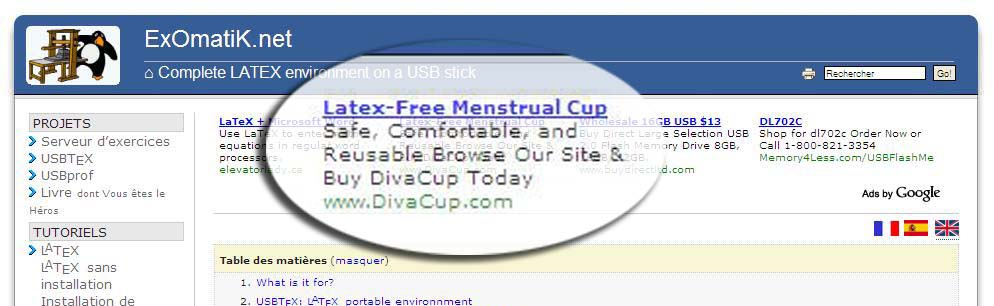
\includegraphics[width=0.9\textwidth]{eg1_LaTeX_vs_Latex_pequeno}

\vfill

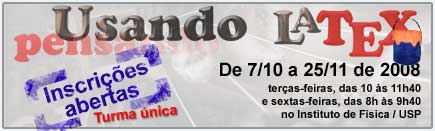
\includegraphics[width=0.5\textwidth]{eg2_LaTeX_vs_Latex}
\end{center}
\end{frame}

%-------------------------------------------------------------------
\logo{}
\begin{frame}[label=word]
\begin{center}
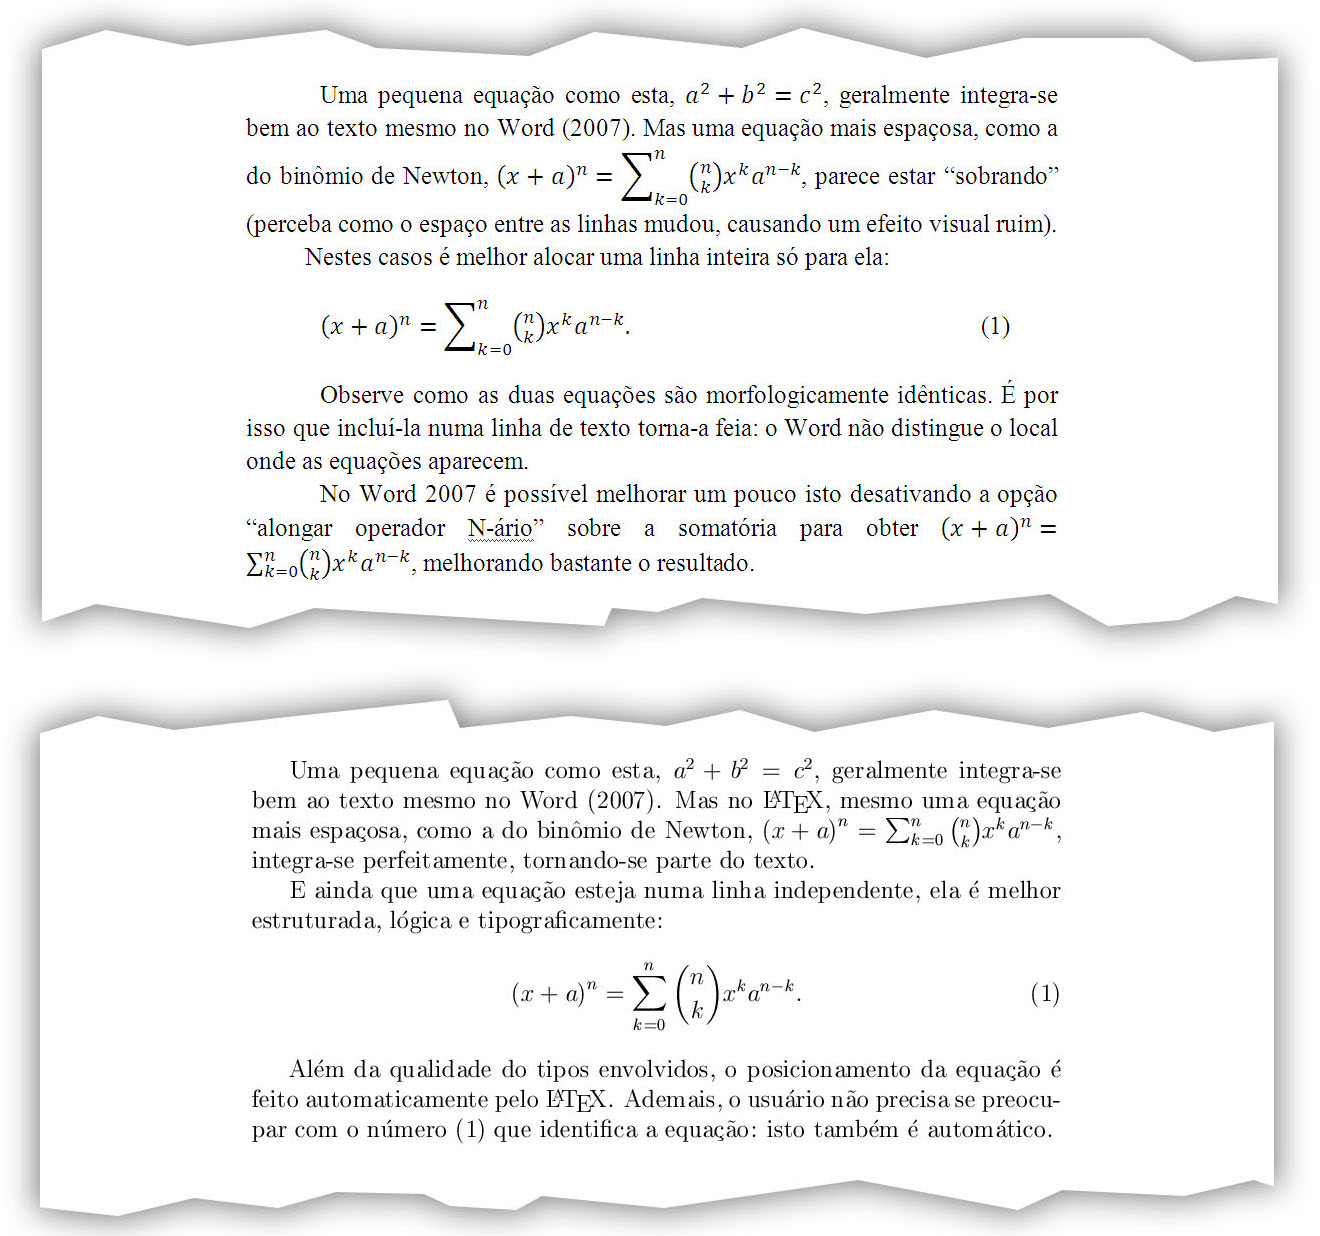
\includegraphics[height=0.9\textheight]{eg_LaTeX_vs_Word}
\end{center}
\end{frame}

\end{document}